\documentclass{article}
\usepackage{amsmath}
\usepackage{currfile}
\usepackage{listings}
\usepackage{xcolor}
\usepackage[utf8]{inputenc}
\usepackage{graphicx}

\definecolor{codegreen}{rgb}{0,0.6,0}
\definecolor{codegray}{rgb}{0.5,0.5,0.5}
\definecolor{codepurple}{rgb}{0.58,0,0.82}
\definecolor{backcolour}{rgb}{0.95,0.95,0.92}

\lstdefinestyle{mystyle}{
    backgroundcolor=\color{backcolour},   
    commentstyle=\color{codegreen},
    keywordstyle=\color{magenta},
    numberstyle=\tiny\color{codegray},
    stringstyle=\color{codepurple},
    basicstyle=\ttfamily\footnotesize,
    breakatwhitespace=false,         
    breaklines=true,                 
    captionpos=b,                    
    keepspaces=true,                 
    numbers=left,                    
    numbersep=5pt,                  
    showspaces=false,                
    showstringspaces=false,
    showtabs=false,                  
    tabsize=2
}

\lstset{style=mystyle}

\title{Oblig1}

\begin{document}

\section*{Kven er med på Gruppa?}

Holly Storøy


\section{Oppgave 1}
%\subsection{Deloppgåve 1.1}

%Klasse "Film" med data, konstruktørar, og metodar
%\lstinputlisting[language=Java]{src/no/hvl/dat102/filmarkiv/impl/Film.java}

%\subsection{Deloppgåve 1.2}
%Grensesnitt  for Filmarkiv
%\lstinputlisting[language=Java]{src/no/hvl/dat102/filmarkiv/adt/FilmarkivADT.java}

%\subsection{Deloppgåve 1.2}
%Grensesnitt  for Filmarkiv
%\lstinputlisting[language=Java]{src/no/hvl/dat102/filmarkiv/adt/FilmarkivADT.java}

%\subsection{Deloppgåve 1.3}
%tabellbasert Implementasjon av Filmarkiv
%\lstinputlisting[language=Java]{src/no/hvl/dat102/filmarkiv/impl/Filmarkiv.java}

%\subsection{Deloppgåve 1.4}
%Filmarkiv JUnit test
%\lstinputlisting[language=Java]{src/no/hvl/dat102/filmarkiv/test/FilmarkivTest.java}

%\subsection{Deloppgåve 1.5}
%FilmarkivMain:
%\lstinputlisting[language=Java]{src/no/hvl/dat102/filmarkiv/impl/FilmarkivMain.java}
%Meny:
%\lstinputlisting[language=Java]{src/no/hvl/dat102/filmarkiv/impl/Meny.java}
%Tekstgrensesnitt:
%\lstinputlisting[language=Java]{src/no/hvl/dat102/filmarkiv/impl/Tekstgrensesnitt.java}

her er sånn programmet ser ut når ein køyrer det.

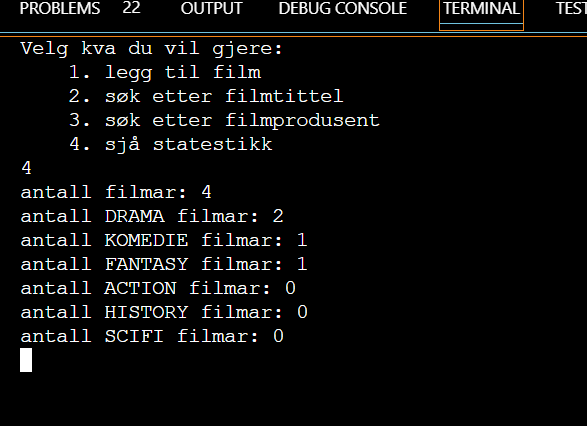
\includegraphics[scale=0.5]{Skjermbilde 2025-01-31 180318.png}

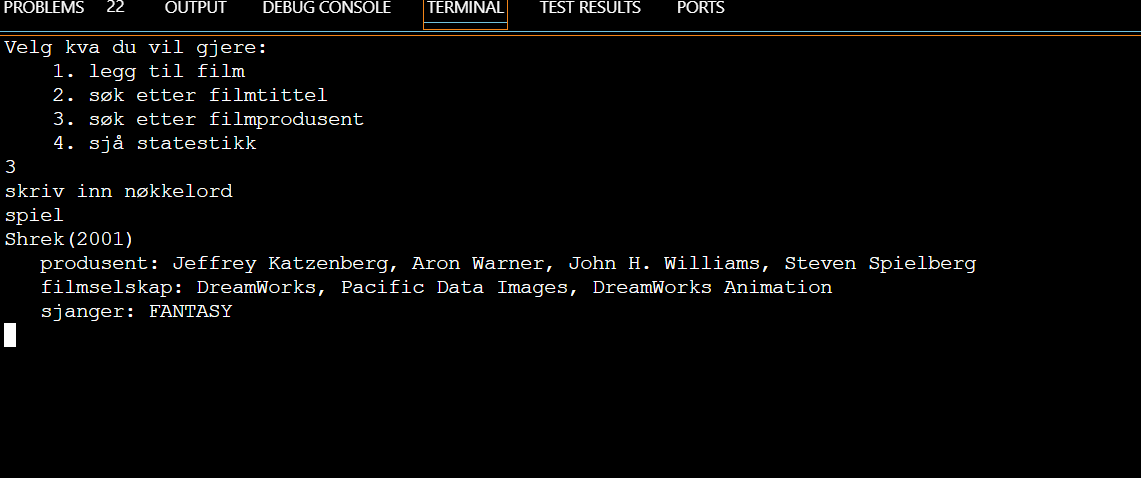
\includegraphics[scale=0.5]{Skjermbilde 2025-01-31 180333.png}

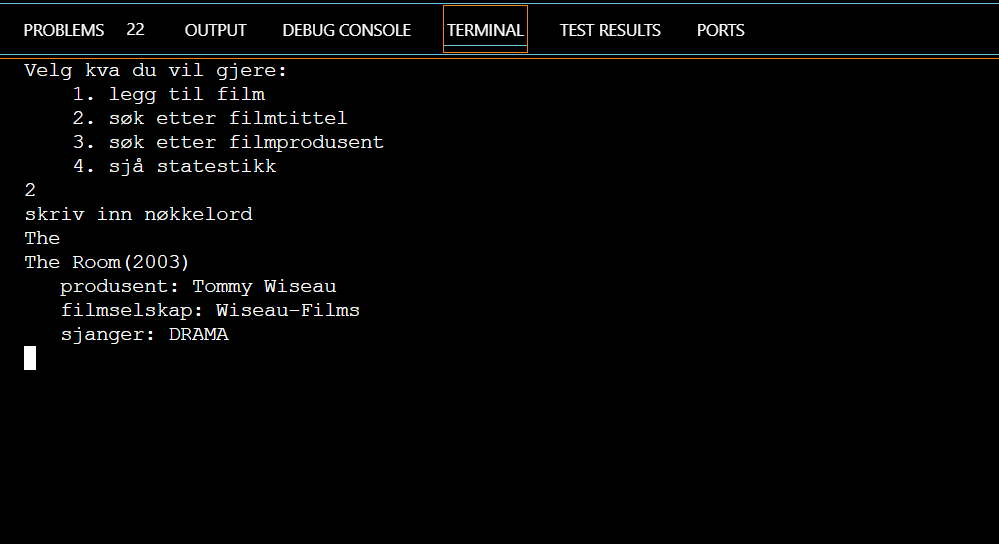
\includegraphics[scale=0.5]{Skjermbilde 2025-01-31 180403.png}

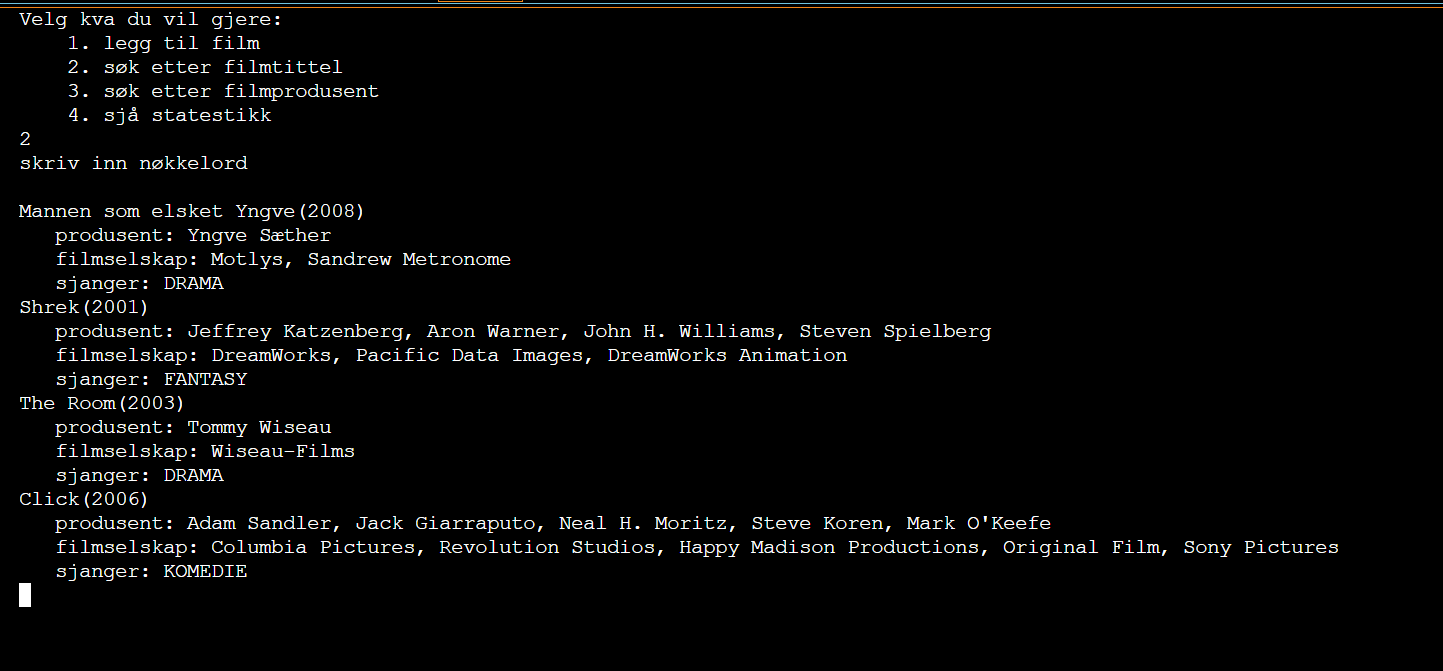
\includegraphics[scale=0.5]{Skjermbilde 2025-01-31 180416.png}

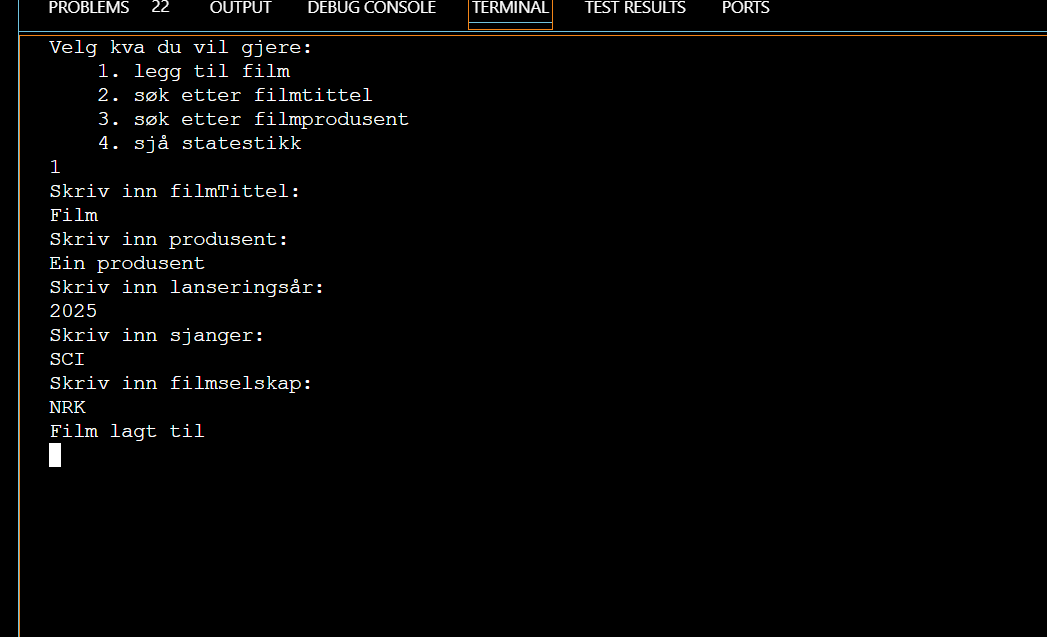
\includegraphics[scale=0.5]{Skjermbilde 2025-01-31 180522.png}

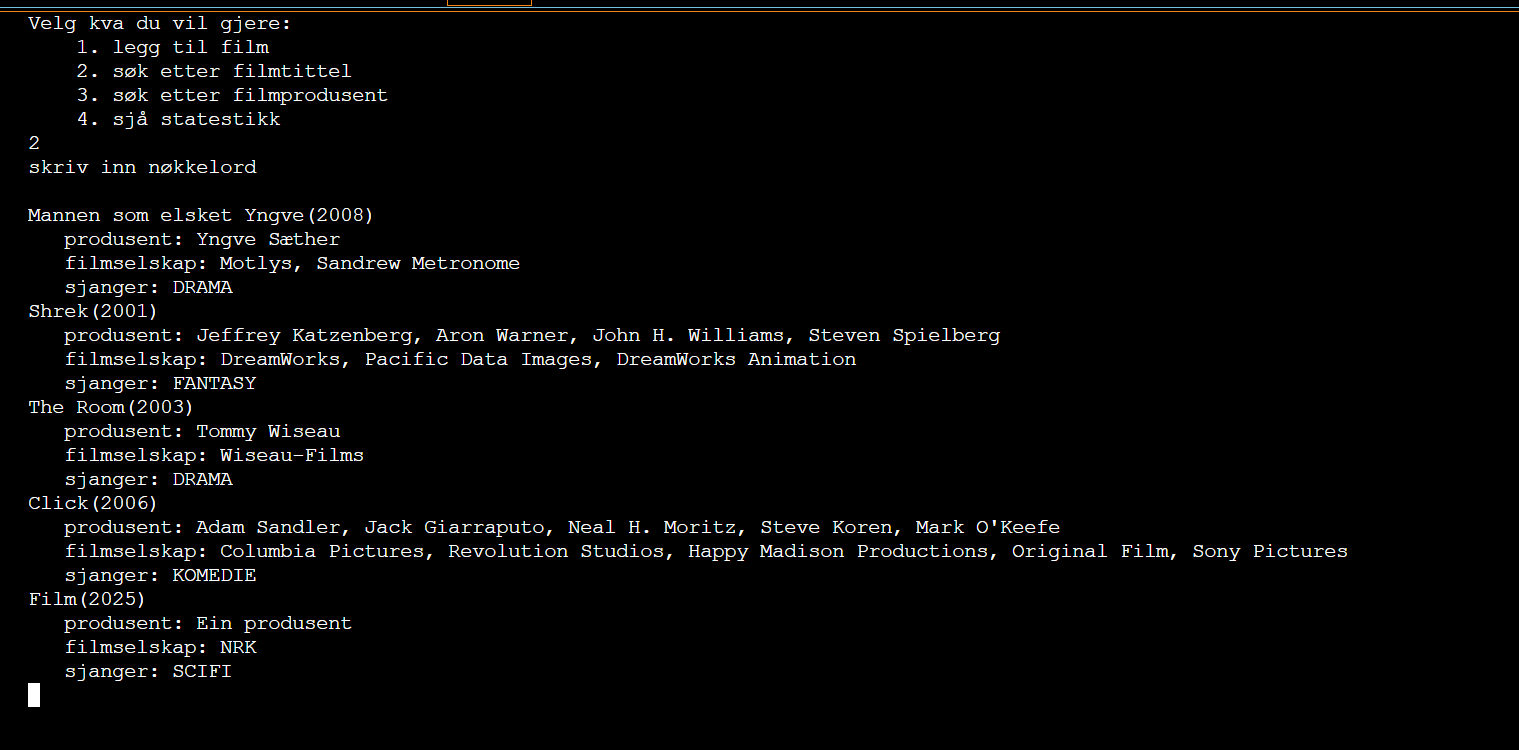
\includegraphics[scale=0.5]{Skjermbilde 2025-01-31 180742.png}

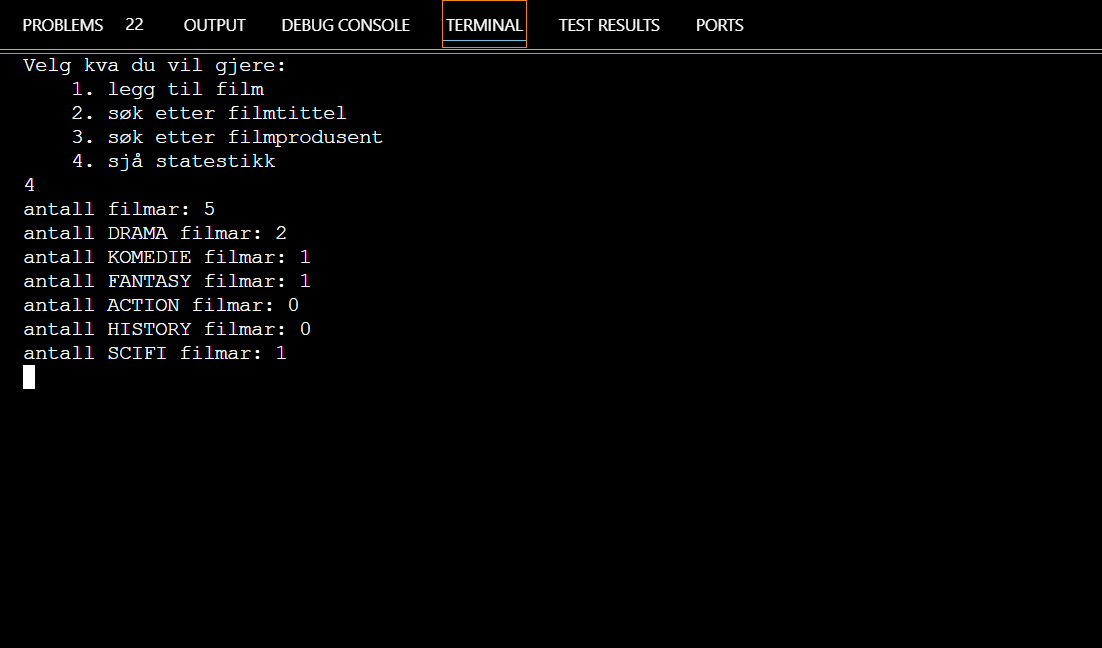
\includegraphics[scale=0.5]{Skjermbilde 2025-01-31 180753.png}


\section{Oppgåve 2}
Her er den nodebaserte implementasjonen av filmarkiv
\lstinputlisting[language=Java]{src/no/hvl/dat102/filmarkiv/impl/Filmarkiv2.java}

ein forskjell som må til når ein bytter implementasjon er å fjerne
inparameteret når ein opretter nytt filmarkiv, sidan den nodebaserte 
implementasjonen ikkje har behov for bestemt lengde


\section{Oppgåve 3}
\subsection{Deloppgåve 3 a)}
\subsubsection*{i.}
$4n^2 + 50n - 10 = O(n^2)$
\subsubsection*{ii.}
$10n + 4 \log_2 n + 30 = O(n)$
\subsubsection*{iii.}
$13n^3 + 22n^2 + 50n + 20 = O(n^3)$
\subsubsection*{iv.}
$35 + 13 \log_2 n = O(log n)$

\subsection{Deloppgåve 3 b)}

mengden tilordningar koden

\begin{lstlisting}[language=Java]
    sum = 0;
    for (int i = n; i > 1; i = i/2) {
        sum = sum + i;
    }
\end{lstlisting}

gjer. Vil gå opp jo større n er, men sidan ein hopper med halvparten av i
per loop, så vil det forholdsvis gå ned i kor mange tilordningar per størrelse på n.
Så tidskompleksiteten blir $O(\log n)$

\subsection{Deloppgåve 3 c)}
\begin{lstlisting}[language=Java]
    sum = 0;
    for (int i = 1; i <= n; i++) {
        for (int j = 1; j <= n; j = j * 2) {
            
        }
    }
\end{lstlisting}

ytterste løkka er ei klassisk for løkke med $O(n)$ kompleksitet.
Den innerste aukar med gange 2, så den $O(\log n)$ 
til sammen får vi då $O(n \log n)$ kompleksitet

\subsection{Deloppgåve 3 d)}
Areal er andregradsfunksjon så den blir $O(n^2)$
omkrets er førestegradsfunksjon, så den blir $O(n)$

\subsection{Deloppgåve 3 f)}

\subsubsection*{i.}
$8n + 4n^3 = O(n^3)$
\subsubsection*{ii.}
$10 \log_2 n + 20 = O(\log n)$
\subsubsection*{iii.}
$20n + 2n \log_2 n + 11 = O(n \log n)$
\subsubsection*{iv.}
$4 \log_2 n + 2n = O(n)$

\subsection*{}

rangert best til verst:
ii $\rightarrow$ iv $\rightarrow$ iii $\rightarrow$ i


\subsection{Deloppgåve 3 g)}
her er koden for målinga
\lstinputlisting[language=Java]{src/oppg3g.java}

her er resultatet eg fikk etter å køyre den nokre gongar

\begin{center}
\begin{tabular}{ |c|c|c| } 
    \hline
    $10^7$ & $10^8$ & $10^9$  \\ 
    \hline
    3ms & 4ms & 17ms \\ 
    0ms & 0ms & 17ms \\ 
    8ms & 9ms & 16ms \\ 
    4ms & 5ms & 18ms \\
    4ms & 4ms & 16ms \\
    \hline
\end{tabular}
\end{center}

vanskeleg å sjå hastigheita $T(n) = cn$ når $10^7$ og $10^8$ 
brukar ca. samme tid, så eg slengte på ein $10^{10}$ og fikk desse resultata

\begin{center}
\begin{tabular}{ |c|c|c|c| } 
        \hline
        $10^7$ & $10^8$ & $10^9$ & $10^{10}$\\ 
        \hline
        0ms & 8ms & 16ms & 164ms \\ 
        3ms & 0ms & 16ms & 172ms \\ 
        4ms & 4ms & 16ms & 163ms \\ 
        4ms & 3ms & 16ms & 173ms \\
        0ms & 0ms & 22ms & 165ms \\
        \hline
\end{tabular}
\end{center}

No ser det meir rikitg ut sida den legger på ca. eit
siffer per $10^x$ 

\end{document}
